%%%%%%%%%%%%%%%%%%%%%%%%%%%%%%%%%%%%%%%%%%%%%%%%%%%%%%%%%%%%%%%%%%%%%%%%%%%%%%%
% Chapter 5 - Chronic Awake Imaging of Photothrombotic Stroke
%%%%%%%%%%%%%%%%%%%%%%%%%%%%%%%%%%%%%%%%%%%%%%%%%%%%%%%%%%%%%%%%%%%%%%%%%%%%%%%

\chapter{Chronic Awake Imaging of Photothrombotic Stroke} \label{ch:awake}

Anesthesia is widely used in preclinical neuroscience research to sedate animals while imaging despite systemic effects on neuronal and vascular function \cite{Janssen:2004ih}. The volatile anesthetic isoflurane has been shown to reduce excitatory synaptic transmission \cite{BergJohnsen:1992wk}, impair oxygen autoregulation \cite{Aksenov:2012wh}, suppress the magnitude and speed of neurovascular coupling \cite{Pisauro:2013cx}, and cause abnormal increases in CBF \cite{Strebel:1995uh, Iida:1998th}. Isoflurane has also been shown to convey neuroprotective effects that may reduce the severity of ischemic lesions \cite{Sakai:2007wc, Burchell:2013tj} and suppress the occurrence and frequency of spreading depolarizations \cite{Kudo:2016ho}. These effects can mask the benefits of neuroprotective agents and potentially impact the outcomes of long-term studies \cite{Kapinya:ua, Seto:2014ga}. Our lab has reported \cite{Ponticorvo:2010uv, Kazmi:2013ey, Sullender:2018ff} conflicting vascular \ce{pO2} measurements that can likely be attributed to the use of different general anesthetics (urethane vs. isoflurane).

The elimination of anesthesia from neuroimaging experiments has grown increasingly popular in recent years with two primary strategies taking the forefront. The first is the usage of head-mounted microscopes that miniaturize many of the optical components into a package that can be installed on the head of the subject \cite{Gu:1999ky, Helmchen:2001tw, Flusberg:2005tq}. While this technique allows for freely-moving tethered imaging, it requires extensive optical engineering and introduces significant motion artifacts caused by normal animal behavior \cite{Helmchen:2001tw}. Miniaturizing the system described in this dissertation would require significant sacrifices in spatial and temporal resolutions for both imaging modalities.

The second strategy involves restraining the animal's head while positioned on a rotating treadmill \cite{Pisauro:2013cx, Dombeck:2007gr, Wienisch:2011ju, Kaifosh:2013fy, Heiney:2018gq} or confined in a small chamber \cite{Silasi:2016dq}, which permits the use of existing imaging platforms. This technique allows for walking or running in place while minimizing motion of the head and imaging region. A spherical treadmill design has been used to perform awake two-photon microscopy with only an estimated 2-5 $\mu$m of lateral motion \cite{Dombeck:2007gr}, which is near the resolution of the dual-modality imaging system. This chapter details the transition from anesthetized to awake animal imaging, including the selection of a treadmill-based restraint system and \textit{in vivo} demonstrations of chronic awake imaging.



%%%%%%%%%%%%%%%%%%%%%%%%%%%%%%%%%%%%%%%%%%%%%%%%%%%%%%%%%%%%%%%%%%%%%%%%%%%%%%%
% Section 5.1 - Awake Imaging System Design
%%%%%%%%%%%%%%%%%%%%%%%%%%%%%%%%%%%%%%%%%%%%%%%%%%%%%%%%%%%%%%%%%%%%%%%%%%%%%%%
\section{Awake Imaging System Design}

The spherical treadmill described by Dombeck \textit{et al.} \cite{Dombeck:2007gr} is a popular design in the neuroscience community. It features a large (8-inch) Styrofoam ball supported on an air cushion produced by a perforated hemispheric casting. The ball allows for two dimensions of free movement, which reduces the torque the animal can apply to its permanently-attached metal headbar that encircles the cranial window. An implementation of this design using a 3D-printed base can be seen in Figure \ref{fig:awakesystems}A. A series of channels spanning the plastic cylinder direct the flow of air upwards to form the supporting air cushion. Flow is regulated using the standard house air supply and can be adjusted as needed depending on the weight of the ball and the subject. While preliminary tests showed the design was functional, the loudness of the flowing air was deemed unsuitable for practical use. The height of the entire apparatus was also a major limitation, with only the dual-modality imaging system capable of the necessary vertical translation.

% Figure - Awake System Designs
\begin{figure}
    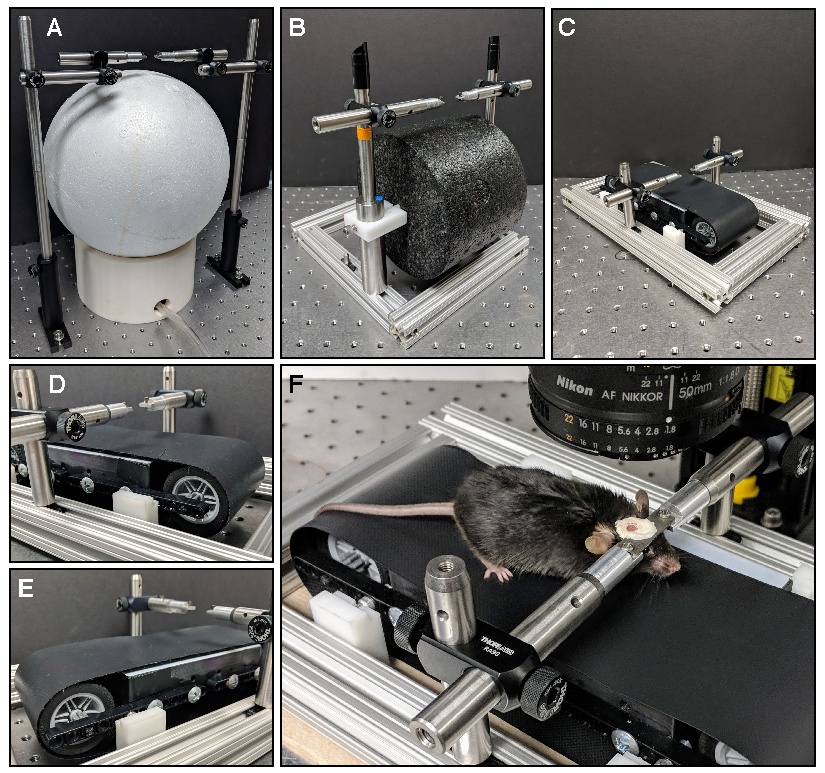
\includegraphics{figures/chapter_5/awakesystems.pdf}
    \caption{
        \label{fig:awakesystems}
        \textbf{(A)} Air-cushioned spherical treadmill, \textbf{(B)} foam wheel treadmill, and \textbf{(C)} low-profile continuous belt treadmill. Close-up of the \textbf{(D)} front and \textbf{(E)} rear pulley wheels on the belt treadmill. \textbf{(F)} Mouse head-restrained on the belt treadmill using the permanently attached headbar.
    }
\end{figure}

Two alternative designs with lower profiles were examined. The first implemented (Figure \ref{fig:awakesystems}B) a rotating foam wheel \cite{Heiney:2018gq} that allowed for one dimension of free movement. The coarse surface of the foam appeared to offer a better grip for the animal than the Styrofoam ball, making it easier to walk. While the vertical height was still substantially greater than the stereotaxic frame used during anesthetized imaging, the apparatus could easily fit under both the dual-modality and standalone MESI systems. However, issues were encountered with the stability of the rotation caused by difficulties in precisely centering the axle through the foam. These rotational variations in the position of the surface of the wheel relative to the headbar caused large motion artifacts in the resulting speckle contrast imagery despite head fixation.

The second design implemented (Figure \ref{fig:awakesystems}C) a continuous belt treadmill \cite{Royer:2012gw, Kaifosh:2013fy} that also allowed for one dimension of self-propelled movement. The rubberized tread rotated over two pulleys made from LEGO tires and axles (Figure \ref{fig:awakesystems}D-E) with the animal centered over a flat piece of plastic. This eliminated the vertical variations that negatively impacted the wheel-based design and resulted in more stable LSCI measurements when the animal moved. The height of the treadmill was also further reduced and only slightly taller than the conventional stereotaxic frame. Figure \ref{fig:awakesystems}F depicts a mouse restrained on the treadmill system via its permanently attached metal headbar (see Appendix \ref{app:headbar_attachment}).



%%%%%%%%%%%%%%%%%%%%%%%%%%%%%%%%%%%%%%%%%%%%%%%%%%%%%%%%%%%%%%%%%%%%%%%%%%%%%%%
% Section 5.2 - Effects of Anesthesia on Hemodynamics
%%%%%%%%%%%%%%%%%%%%%%%%%%%%%%%%%%%%%%%%%%%%%%%%%%%%%%%%%%%%%%%%%%%%%%%%%%%%%%%
\section{Effects of Anesthesia on Hemodynamics}

\textit{In vivo} imaging with the head-restrained treadmill system was demonstrated by comparing awake and anesthetized hemodynamics. The subject was mounted on the treadmill using its headbar and allowed to acclimate for 10-15 minutes prior to imaging. The mounting rods were adjusted as necessary to maintain a comfortable head position and to orient the cranial window perpendicularly to the optical axis. Subjects quickly adapted to walking on the treadmill and would exhibit regularly grooming behavior when stationary.

%%%%%%%%%%%%%%%%%%%%%%%%%%%%%%%%%%%%%%%%%%%%%%%%%%%%%%%%%%%%%%%%%%%%%%%%%%%%%%%
\subsection{Dynamic Cerebral Blood Flow} \label{ssec:dynamicawakecbf}

An extended MESI acquisition was performed on the standalone MESI system to monitor the stability of awake and anesthetized measurements and the transition between the two states. The awake subject was imaged continuously for one hour with a nose-cone placed directly in front of the restrained animal and delivering only medical air. General anesthesia was then quickly induced with medical air vaporized isoflurane (2.5\%) via the nose-cone. After several minutes, the isoflurane was reduced to 1.5\% and a feedback heating pad (DC Temperature Controller, FHC) placed under the animal to regulate body temperature. The anesthetized subject was imaged for an additional one hour before being removed from anesthesia and allowed to recover on the heating pad.

% Figure - Speckle Awake vs. Anesthetized
\begin{figure}
    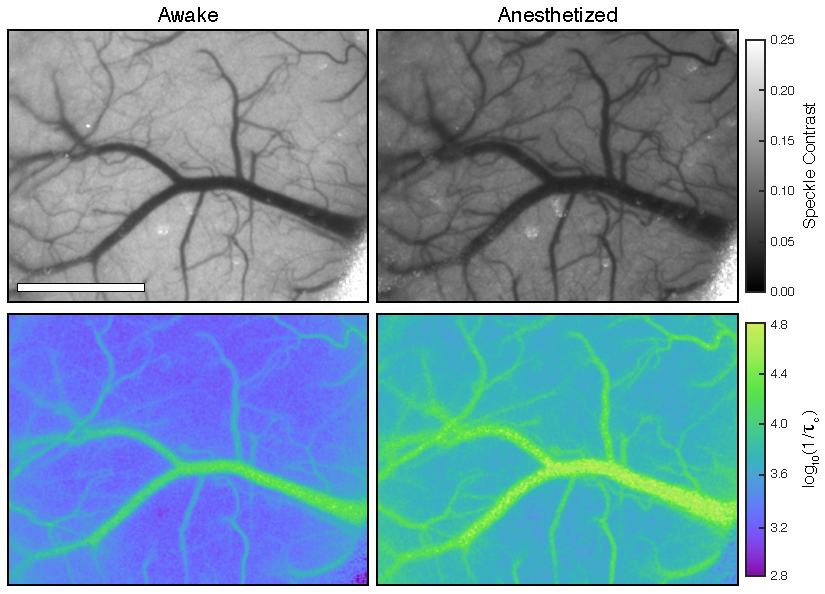
\includegraphics{figures/chapter_5/speckleawakeanes.pdf}
    \caption{
        \label{fig:speckleawakeanes}
        Speckle contrast (top) and MESI ICT (bottom) imagery from a mouse while awake (left) and anesthetized (right) exhibits the systemic change in CBF (Scale bar = 1 mm).
    }
\end{figure}

Figure \ref{fig:speckleawakeanes} depicts averaged single-exposure (5 ms) speckle contrast images and their corresponding MESI ICT images during the awake and anesthetized states. Anesthesia caused a systematic increase in CBF as exhibited by the decrease in average speckle contrast (0.199 $\to$ 0.166) and increase in average ICT (2798 $s^{-1} \to$ 6579 $s^{-1}$). Significant vasodilation can also be seen in the large central vein and the many smaller vessels that only become visible in the anesthetized state. These results are consistent with volatile anesthetics being potent vasodilators that cause dose-dependent increases in baseline CBF uncoupled from local metabolic demands \cite{Masamoto:2012bj}.

Figure \ref{fig:flowawakeanes}A highlights two vascular regions (R1, R2) and one parenchyma region (R3) analyzed over the entire awake-to-anesthetized MESI acquisition. While the head-restraint minimized most undesired motion, \texttt{elastix} was used during post-processing to rigidly align all speckle contrast frames to the beginning of the acquisition. Figure \ref{fig:flowawakeanes}B depicts the resulting relative blood flow timecourses using the average of the entire one hour of awake imaging as the ICT baseline. Flow was stable throughout the awake imaging segment with occasional spikes corresponding to animal motion. However, it is difficult to determine whether these are real changes in blood flow or if the physical motion itself is causing the change in $\tau_c$. The induction of general anesthesia rapidly caused a 3x increase in relative flow across all three ROIs before reaching a semi-stable state after about 10 minutes. The spike around $t$ = 5000 seconds was likely caused by an unstable anesthesia plane or difficulty with breathing resulting in increased animal motion. However, this quickly subsided and the flow remained relatively stable as it slightly declined to around 2.5x of baseline in all three ROIs over the remainder of the imaging session.

% Figure - Awake to Anesthetized Timecourses
\begin{figure}
    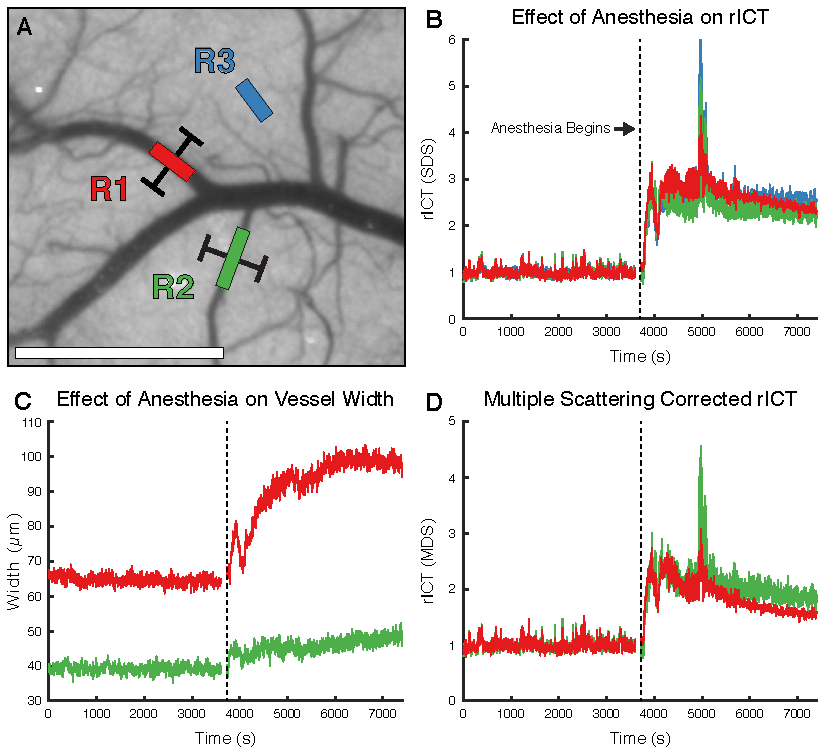
\includegraphics{figures/chapter_5/flowawakeanes.pdf}
    \caption{
        \label{fig:flowawakeanes}
        \textbf{(A)} MESI ICT was calculated within two branches of a large central vein (R1 and R2) and a parenchyma region (R3) as a mouse was anesthetized (Scale bar = 1 mm). \textbf{(B)} Relative ICT timecourses over one hour of awake imaging followed by one hour of anesthetized imaging. \textbf{(C)} Estimated diameters of R1 and R2 over the imaging session. \textbf{(D)} Relative ICT timecourses using the multiple dynamic scattering MESI model.
    }
\end{figure}

In order to examine anesthesia-induced vasodilation, the diameters of both vessels (R1, R2) were estimated from the speckle contrast images. Cross-sectional profiles (the black bars in Figure \ref{fig:flowawakeanes}A) averaged over the length of each ROI were fitted to a Gaussian distribution. The vessel diameter was defined as the full width at half maximum (FWHM) of the fitted cross-section. The FWHM was computed for both vessels in every frame of the acquired data and is shown in Figure \ref{fig:flowawakeanes}C. Similar to the relative flow within the ROIs, the diameters remained stable throughout the entire awake imaging segment. However, the induction of anesthesia caused significant vasodilation in vessel R1 (+54\%) while vessel R2 increased slightly (+23\%) over the entire anesthetized imaging segment. The reason for this discrepancy is unclear, especially since the imagery in Figure \ref{fig:speckleawakeanes} appears to show systemic vasodilation. The use of speckle contrast images for estimating the vessel diameter is a somewhat ill-posed problem since the technique has reduced spatial resolution compared to a conventional reflectance image.

As discussed in Chapter \ref{ch:mesi}, the standard MESI model represented by Equation \ref{eq:mesi} assumes that detected photons only experience single dynamic scattering interactions and the underlying particle motion has a Lorentzian velocity distribution indicative of Brownian motion \cite{Parthasarathy:2008el}. However, camera pixels corresponding to resolvable surface vasculature are more likely to sample photons that have experienced multiple dynamic scattering events \cite{Davis:2014kc} and exhibit Gaussian velocity distributions indicative of bulk flow \cite{Kazmi:2015du}. The single dynamic scattering correlation time ($\tau_c^{sds}$) can be converted to the multiple dynamic scattering correlation time ($\tau_c^{mds}$) by scaling the former by the average number of dynamic scattering events ($N_d$), which is proportional to the vessel diameter \cite{Kazmi:2015du}. Figure \ref{fig:flowawakeanes}D plots the ``corrected'' relative ICT$_{mds}$ that accounts for multiple scattering events using the vessel width data from Figure \ref{fig:flowawakeanes}C. This new estimate shows a slightly reduced 2.5x increase in flow during anesthesia in the vascular ROIs compared to the 3x increase seen with relative ICT$_{sds}$. It also reveals a more substantial decrease in flow over the remainder of the anesthetized imaging session down to only 1.5x of baseline.

%%%%%%%%%%%%%%%%%%%%%%%%%%%%%%%%%%%%%%%%%%%%%%%%%%%%%%%%%%%%%%%%%%%%%%%%%%%%%%%
\subsection{Static Cerebral Blood Flow and Oxygen Tension}

MESI and \ce{pO2} measurements were performed on the dual-modality imaging system to examine the behavior of the two hemodynamic parameters in the awake and anesthetized states. The subject was briefly anesthetized to administer Oxyphor PtG4 via retro-orbital injection for a target blood plasma concentration of 5 $\mu$M and allowed to recover for two hours before being placed on the treadmill. Static MESI and 445 nm \ce{pO2} measurements were acquired from the ROIs shown in Figure \ref{fig:specklepO2awakeanes}A covering one arteriole (A1), three veins (V1, V2, V3), and one parenchyma region (P1). The subject was then anesthetized in place via nose cone inhalation of medical air vaporized isoflurane (1.5\%) and another set of MESI and 445 nm \ce{pO2} measurements acquired after 15 minutes.

% Figure - Awake and Anesthetized Static MESI ICT and pO2
\begin{figure}
    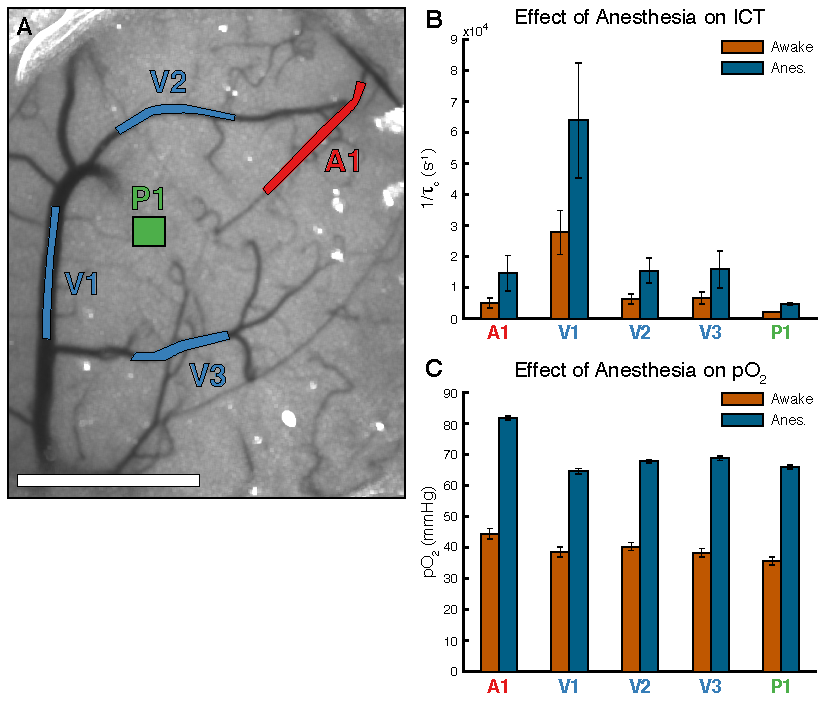
\includegraphics{figures/chapter_5/specklepO2awakeanes.pdf}
    \caption{
        \label{fig:specklepO2awakeanes}
        \textbf{(A)} Awake single-exposure speckle contrast image overlaid with regions targeted for ICT and \ce{pO2} measurements (Scale bar = 1 mm). One arteriole (A1), three veins (V1, V2, V3), and one parenchyma region (P1) were examined. The ROIs covered areas between 0.028-0.039 mm$^2$. \textbf{(B)} MESI ICT and \textbf{(C)} 445 nm \ce{pO2} measurements within the targeted regions during awake and anesthetized states (mean $\pm$ s.d.).
    }
\end{figure}

Figure \ref{fig:specklepO2awakeanes}B shows the change in MESI ICT within each of the ROIs between the awake and anesthetized states. Similar to the results shown in Section \ref{ssec:dynamicawakecbf}, there was a 2.5x increase in relative flow while under general anesthesia. The \ce{pO2} measurements also experienced a systematic increase when in the anesthetized state (Figure \ref{fig:specklepO2awakeanes}C). The awake \ce{pO2} is significantly lower than the values reported in Section \ref{sec:acutedemo} and the arteriole only exhibits a marginally higher \ce{pO2} compared to the other regions. These results are similar to the findings of Lyons \textit{et al.} \cite{Lyons:2016bd}, who reported a mean capillary \ce{pO2} of 36 mmHg in the cortex and suggested that the increase in \ce{pO2} during anesthesia is caused by the increase in blood flow.



%%%%%%%%%%%%%%%%%%%%%%%%%%%%%%%%%%%%%%%%%%%%%%%%%%%%%%%%%%%%%%%%%%%%%%%%%%%%%%%
% Section 5.3 - Awake Targeted Photothrombosis Induction
%%%%%%%%%%%%%%%%%%%%%%%%%%%%%%%%%%%%%%%%%%%%%%%%%%%%%%%%%%%%%%%%%%%%%%%%%%%%%%%
\section{Awake Targeted Photothrombosis Induction}

Targeted photothrombosis was demonstrated in an awake mouse while simultaneously monitoring CBF and \ce{pO2} (Figure \ref{fig:acuteawakephotothrombosis}). The subject was briefly anesthetized on the treadmill via nose-cone inhalation of isoflurane (3.0\%) in order to administer rose bengal (50 $\mu$L, 15 mg/mL) via retro-orbital injection. Anesthesia was immediately stopped and the nose-cone removed, with the animal regaining consciousness after about three minutes. A descending arteriole (Figure \ref{fig:acuteawakephotothrombosis}A) was targeted at $t$ = 90 seconds with DMD-patterned green light for 10 minutes to induce a photothrombotic occlusion. 445 nm \ce{pO2} measurements were continuously acquired from the stroke target region at 1 Hz with 2500 decays averaged per record. The series of speckle contrast images depict the progression of photothrombosis with the targeted vessel fully occluding after less than three minutes of exposure. \texttt{elastix} was again used during post-processing to rigidly align all speckle contrast frames to the beginning of the acquisition.

% Figure - Acute Awake Photothrombosis
\begin{figure}
    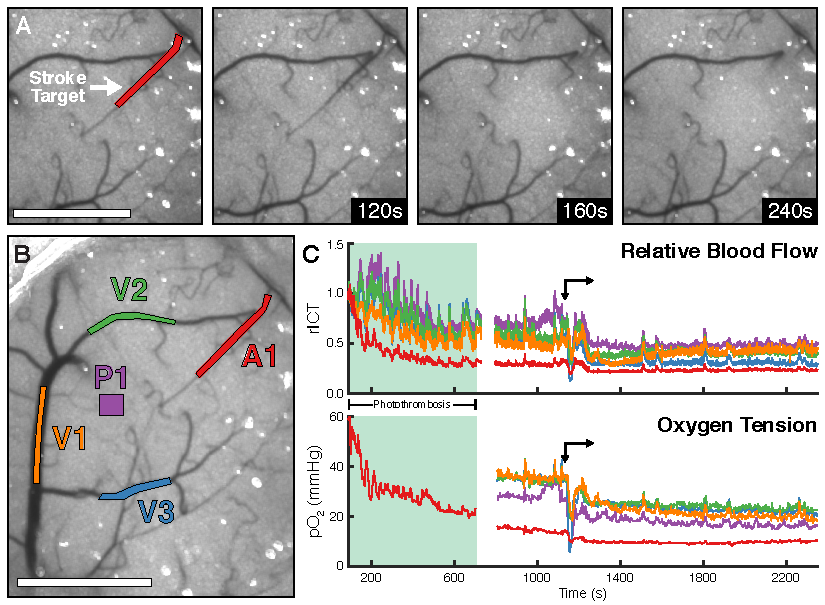
\includegraphics{figures/chapter_5/acuteawakephotothrombosis.pdf}
    \caption{
        \label{fig:acuteawakephotothrombosis}
        \textbf{(A)} Single-exposure speckle contrast images depicting the occlusion of a descending arteriole using DMD-targeted photothrombosis. The red overlay indicates the 0.06 mm$^2$ region simultaneously illuminated for occlusion and \ce{pO2} measurements. \textbf{(B)} One arteriole (A1), three veins (V1, V2, V3), and one parenchyma region (P1) were targeted for \ce{pO2} measurements after stroke induction. \textbf{(C)} Relative blood flow and \ce{pO2} within the targeted regions during and after photothrombosis. The green-shaded section indicates irradiation of the targeted arteriole. The gap in data occurred because of technical difficulties. The arrows indicate the propagation of an ischemia-induced depolarization event (Scale bars = 1 mm).
    }
\end{figure}

Figure \ref{fig:acuteawakephotothrombosis}B depicts the five regions (one arteriole, three veins, and one parenchyma) monitored for dynamic relative blood flow and \ce{pO2} measurements. The arteriole region (A1) is the same vessel targeted for photothrombotic occlusion. ROI \ce{pO2} measurements were initiated shortly after the end of photothrombosis irradiation with patterns displayed at 2 Hz with 1250 decays averaged per record. The resulting timecourses of relative blood flow and \ce{pO2} can be seen in Figure \ref{fig:acuteawakephotothrombosis}C. Compared to the anesthetized photothrombosis measurements in Section \ref{sec:photothrombosis_induction}, these timecourses are significantly more variable because of walking and other animal motions. However, the subject had no visible reaction to the photothrombosis. By $t$ = 200 seconds, flow within the targeted arteriole had decreased to \textless50\% of baseline and \ce{pO2} had dropped from 60 mmHg to around 30 mmHg. However, the animal was likely still experiencing the effects of anesthesia, making it impossible to attribute the changes exclusively to the photothrombotic occlusion.

The propagation of an ischemia-induced depolarization event can be seen beginning at $t$ = 1150 seconds, with sharp reductions in both relative blood flow and \ce{pO2} across all ROIs. The magnitude of these changes are smaller than those seen in the anesthetized data (Figure \ref{fig:photothrombosisacute}C), which is consistent with the results of a calcium imaging study performed during awake ischemic stroke \cite{Balbi:2017cj}. As the depolarization subsided, flow within the targeted arteriole further decreased to \textless20\% of baseline while the \ce{pO2} dropped to only 10 mmHg. Flow and \ce{pO2} in all other regions remained depressed following the depolarization and were relatively steady until the end of the 40-minute imaging session. There was also a reduction in animal motion compared to pre-depolarization behavior as seen by the lack of regular spikes in relative blood flow.



%%%%%%%%%%%%%%%%%%%%%%%%%%%%%%%%%%%%%%%%%%%%%%%%%%%%%%%%%%%%%%%%%%%%%%%%%%%%%%%
% Section 5.4 - Chronic Awake Post-Stroke Hemodynamics
%%%%%%%%%%%%%%%%%%%%%%%%%%%%%%%%%%%%%%%%%%%%%%%%%%%%%%%%%%%%%%%%%%%%%%%%%%%%%%%
\section{Chronic Awake Post-Stroke Hemodynamics}

The chronic progression of the ischemic lesion was monitored using awake imaging for eight days following photothrombosis. Anesthesia was not utilized in any of the post-photothrombosis imaging sessions. Data was only acquired when the animal was completely stationary because motion could interfere with the measurements and the resulting hemodynamic response would not be indicative of the resting state. The perfusion of the occluded arteriole and broader effects on cortical flow were tracked using 5 ms single-exposure LSCI (Figure \ref{fig:chronicawakephotothrombosis}A) and MESI ICT (Figure \ref{fig:chronicawakephotothrombosis}B). Tiled \ce{pO2} maps acquired using 445 nm excitation reveal the spatial extent of the oxygen deficit and subsequent recovery (Figure \ref{fig:chronicawakephotothrombosis}C). The broad range of \ce{pO2} values covered by the colormap masks the smaller differences between arterioles and veins that can be seen on Day -0. The gradient between the occluded vessel and the surrounding tissue diminishes over the course of Days +1, +2, and +3 as the occluded arteriole begins to reperfuse. By Day +5, the vessel had fully reperfused leaving little evidence of the infarct in the speckle contrast or ICT imagery while the tiled \ce{pO2} maps reveal a region of increased oxygenation surrounding the formerly occluded vessel. However, the distal \ce{pO2} measurements also appear to have increased, suggesting this change may be systemic.

% Figure - Chronic Awake Photothrombosis
\begin{figure}
    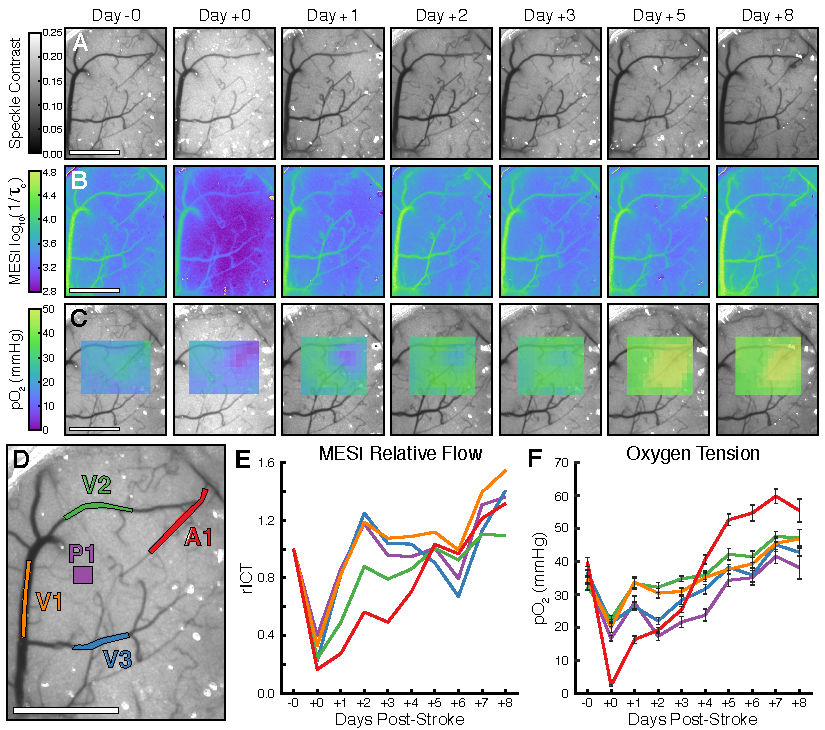
\includegraphics{figures/chapter_5/chronicawakephotothrombosis.pdf}
    \caption{
        \label{fig:chronicawakephotothrombosis}
        Progression of the ischemic lesion over eight days as imaged with \textbf{(A)} single-exposure LSCI, \textbf{(B)} MESI ICT, and \textbf{(C)} 445 nm tiled \ce{pO2} measurements. Day -0 measurements were taken immediately prior to photothrombosis induction and Day +0 measurements were taken immediately after. \textbf{(D)} One arteriole (A1), three veins (V1), and one parenchyma region (P1) were targeted for chronic \textbf{(E)} relative blood flow and \textbf{(F)} 445 nm \ce{pO2} measurements (mean $\pm$ s.d.). Relative MESI ICT was baselined against Day -0 measurements (Scale bars = 1 mm).
    }
\end{figure}

The same five regions (one arteriole, three veins, and one parenchyma) used during the acute awake photothrombosis measurements were also targeted for chronic relative blood flow and 445 nm \ce{pO2} measurements (Figure \ref{fig:chronicawakephotothrombosis}D-F). The relative blood flow was calculated using the pre-stroke (Day -0) MESI ICT measurements as the baseline. The first post-stroke measurements (Day +0) were taken immediately after the conclusion of the photothrombosis induction and reveal systemic deficits in both blood flow and \ce{pO2} likely caused by the spreading depolarization. Blood flow within the targeted arteriole (A1) and a nearby vein (V2) slowly recovered over the course of five days while the remaining ROIs experienced a slight overshoot in relative flow during the same period. Flow continued to increase across all ROIs over the remaining three days and was elevated over baseline by the final imaging session on Day +8. Similar results are seen in the \ce{pO2} measurements, with only A1 experiencing a significant decline from pre-stroke values and the \ce{pO2} increasing across all ROIs over the eight days of imaging. A1 also exhibits the elevated \ce{pO2} seen in the tiled maps (Figure \ref{fig:chronicawakephotothrombosis}C) beginning on Day +5.

The speed of the recovery from the photothrombotic infarct is similar to the anesthetized results (Section \ref{sec:chronic_hemodynamics}) and faster than previous studies in the lab \cite{Schrandt:2015gu}. The targeted arteriole remained occluded for three days following photothrombosis before fully reperfusing. During this period, another arteriole approaching from midline (bottom of the camera FOV) hyperperfused and likely served as a collateral blood supply to mitigate the severity of the flow deficit. Once flow was restored to the targeted vessel on Day +4, the collateral arteriole returned to near baseline flow. Creating a larger infarct would have required targeted both arterioles with the DMD to more severely reduce flow to the region.



%%%%%%%%%%%%%%%%%%%%%%%%%%%%%%%%%%%%%%%%%%%%%%%%%%%%%%%%%%%%%%%%%%%%%%%%%%%%%%%
% Section 5.5 - Discussion
%%%%%%%%%%%%%%%%%%%%%%%%%%%%%%%%%%%%%%%%%%%%%%%%%%%%%%%%%%%%%%%%%%%%%%%%%%%%%%%
\section{Discussion}

The transition to fully awake imaging eliminates the systemic effects of general anesthesia. The potent vasodilation \cite{Iida:1998th} and suppression of neurovascular coupling \cite{Pisauro:2013cx} caused by isoflurane is a significant confounding variable when studying chronic cortical hemodynamics. The head-restrained treadmill design using a continuous linear belt allows for awake imaging while minimizing animal motion that could disrupt the optical measurements. \textit{In vivo} awake imaging was demonstrated with the apparatus using both the dual-modality and standalone MESI systems. Comparisons with anesthetized imaging highlighted the systemic effects of isoflurane of cerebral hemodynamics, with both blood flow and \ce{pO2} more than doubling under general anesthesia.

Despite the efficacy of the head restraint system, correlation time estimates with LSCI remain extremely sensitive to any motion within the imaging area. The animal walking would cause abrupt spikes in ICT that could not definitively be ascribed to neurovascular coupling instead of just a slight motion-related displacement. Excluding data during these periods of heightened activity offers the simplest solution for acquiring reliable instantaneous measurements of blood flow. However, if the hemodynamic response itself is being studied, then further measures would need to be taken in order to more robustly restrict motion of the brain.

The induction of a DMD-targeted photothrombotic occlusion produced similar results to the anesthetized demonstration in Section \ref{sec:photothrombosis_induction}. However, the induction procedure still required the brief use of anesthesia for the injection of the photothrombotic agent. While it is unclear what minimum dosage of isoflurane is needed to convey its neuroprotective effects \cite{Kapinya:ua}, the photothrombosis was performed under the lingering influence of isoflurane. This obfuscates the true changes in blood flow and \ce{pO2} caused by the photothrombotic occlusion itself. Transitioning to a tail vein or intraperitoneal injection prior to mounting on the treadmill would allow for the complete elimination of isoflurane from the stroke induction process.

The resulting infarct was less severe than the anesthetized demonstration and was likely mitigated by the availability of collateral blood supply. The timeline for reperfusion of the targeted vessel was similar to that of the anesthetized chronic imaging (Section \ref{sec:chronic_hemodynamics}) with a full recovery after five days. The use of MESI allowed for more robust estimates of $\tau_c$ and therefore more reliable day-to-day comparisons of blood flow than traditional single-exposure LSCI. Combined with the absolute measurements of \ce{pO2}, the dual-modality imaging system facilitates the chronic study of ischemia in awake animals.



%%%%%%%%%%%%%%%%%%%%%%%%%%%%%%%%%%%%%%%%%%%%%%%%%%%%%%%%%%%%%%%%%%%%%%%%%%%%%%%
% END Chapter 5
%%%%%%%%%%%%%%%%%%%%%%%%%%%%%%%%%%%%%%%%%%%%%%%%%%%%%%%%%%%%%%%%%%%%%%%%%%%%%%%
